


\begin{frame}[fragile]{Kernel Interaction}

 \begin{block}{Composability}
   \begin{itemize}
    \item Mix and match functionality in different libraries
    \item Basic entity: function calls
   \end{itemize}
 \end{block}
 
% Motivating example: sort
 %\pause
 \begin{block}{Example: Sorting}
  \begin{lstlisting}
 void sort_criterion(...) { /* tricky criterion */ }
 std::sort(x.begin(), x.end(), sort_criterion);
  \end{lstlisting}
 \end{block}

  %\pause
  \begin{block}{OpenCL on CPU}
   \begin{itemize}
    \item Plethora of libraries for host available
    \item Easy to call OpenCL libraries from host
    \item (Almost) Impossible to call host libraries from OpenCL kernel
   \end{itemize}
 \end{block}
 
\end{frame}


% Show figure: Diode effect of OpenCL

\begin{frame}[fragile]{Kernel Interaction}

\begin{center}
  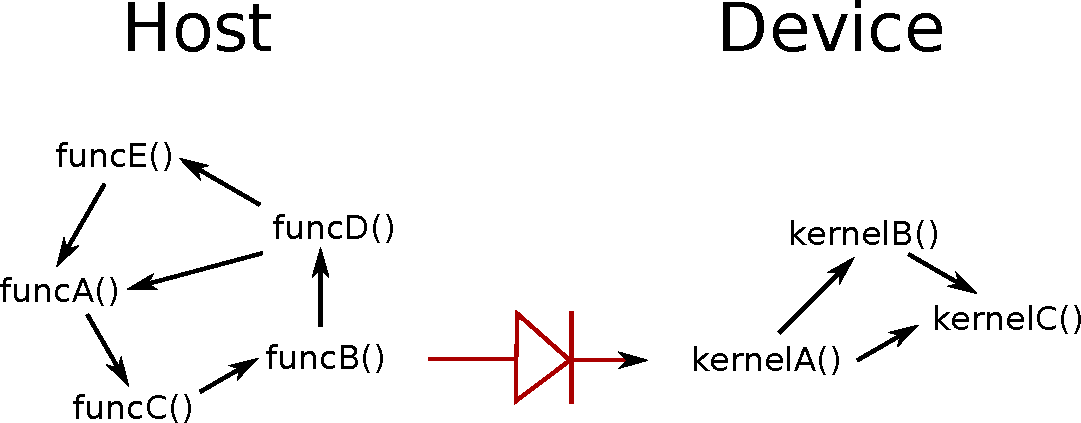
\includegraphics[width=0.9\textwidth]{figures/diode}
\end{center}

 %\pause
 \begin{block}{Proposed Improvement}
   \begin{itemize}
    \item Allow calling host functions for OpenCL kernels on CPU
   \end{itemize}
 \end{block}
  
\end{frame}
